\documentclass[11pt]{article}

% Language setting
% Replace `english' with e.g. `spanish' to change the document language
\usepackage[german]{babel}
% Set page size and margins
% Replace `letterpaper' with`a4paper' for UK/EU standard size
\usepackage[a4paper,top=2cm,bottom=2cm,left=2cm,right=2cm,marginparwidth=1.75cm]{geometry}
\linespread{1.15}
\usepackage{rotating}

% Entferne Einrückungen
\setlength{\parindent}{0in}

% Useful packages
\usepackage[T1]{fontenc}
\usepackage{amsmath}
\usepackage{graphicx}
\usepackage[colorlinks=true, allcolors=blue]{hyperref}
\usepackage[utf8]{inputenc}
\usepackage{todonotes}
\usepackage{listings}
\usepackage{color}
\usepackage{svg}
\usepackage{tabularx}
\usepackage[official]{eurosym}
\usepackage{pdfpages}
\usepackage{microtype}
\usepackage{booktabs} % Für schönere Listen
\usepackage[official]{eurosym} % Für Eurozeichen
\DeclareUnicodeCharacter{20AC}{\euro} % € wird als \euro interpretiert
%%%%%%%%%%%%%%%%%%%%%%%%%%%%%%%%%%%%%%%%%%%%%%%%%%%%%%%%%%%%%%
% See https://latex.org/forum/viewtopic.php?t=1735
\usepackage{makeidx}
\makeindex

\makeatletter
\let\thedate\@date
\makeatother

%%%%%%%%%%%%%%%%%%%%%%%%%%%%%%%%%%%%%%%%%%%%%%
% Begin
%%%%%%%%%%%%%%%%%%%%%%%%%%%%%%%%%%%%%%%%%%%%%%
\begin{document}
\pagenumbering{Roman}
\begin{titlepage}
    \begin{center}
        \vspace*{3cm}
            
        \Huge
        \textbf{Angebot}
            
        \vspace{0.5cm}
        \LARGE
        "Dog Royale"
            
        \vspace{1.5cm}
            
        \textbf{Softwaretechnikpraktikum Gruppe 1}
        
        \Large
        \thedate\\
        
            
        \vfill
        
\includegraphics[width=.5\textwidth]{images/Logo_Uni_Paderborn.pdf}
        
    \end{center}
\end{titlepage}
%%%%%%%%%%%%%%%%%%%%%%%%%%%%%%%%%%%%%%%%%%%%%%
% Table of contents
%%%%%%%%%%%%%%%%%%%%%%%%%%%%%%%%%%%%%%%%%%%%%%
\clearpage
\tableofcontents
\thispagestyle{empty}
%\newpage
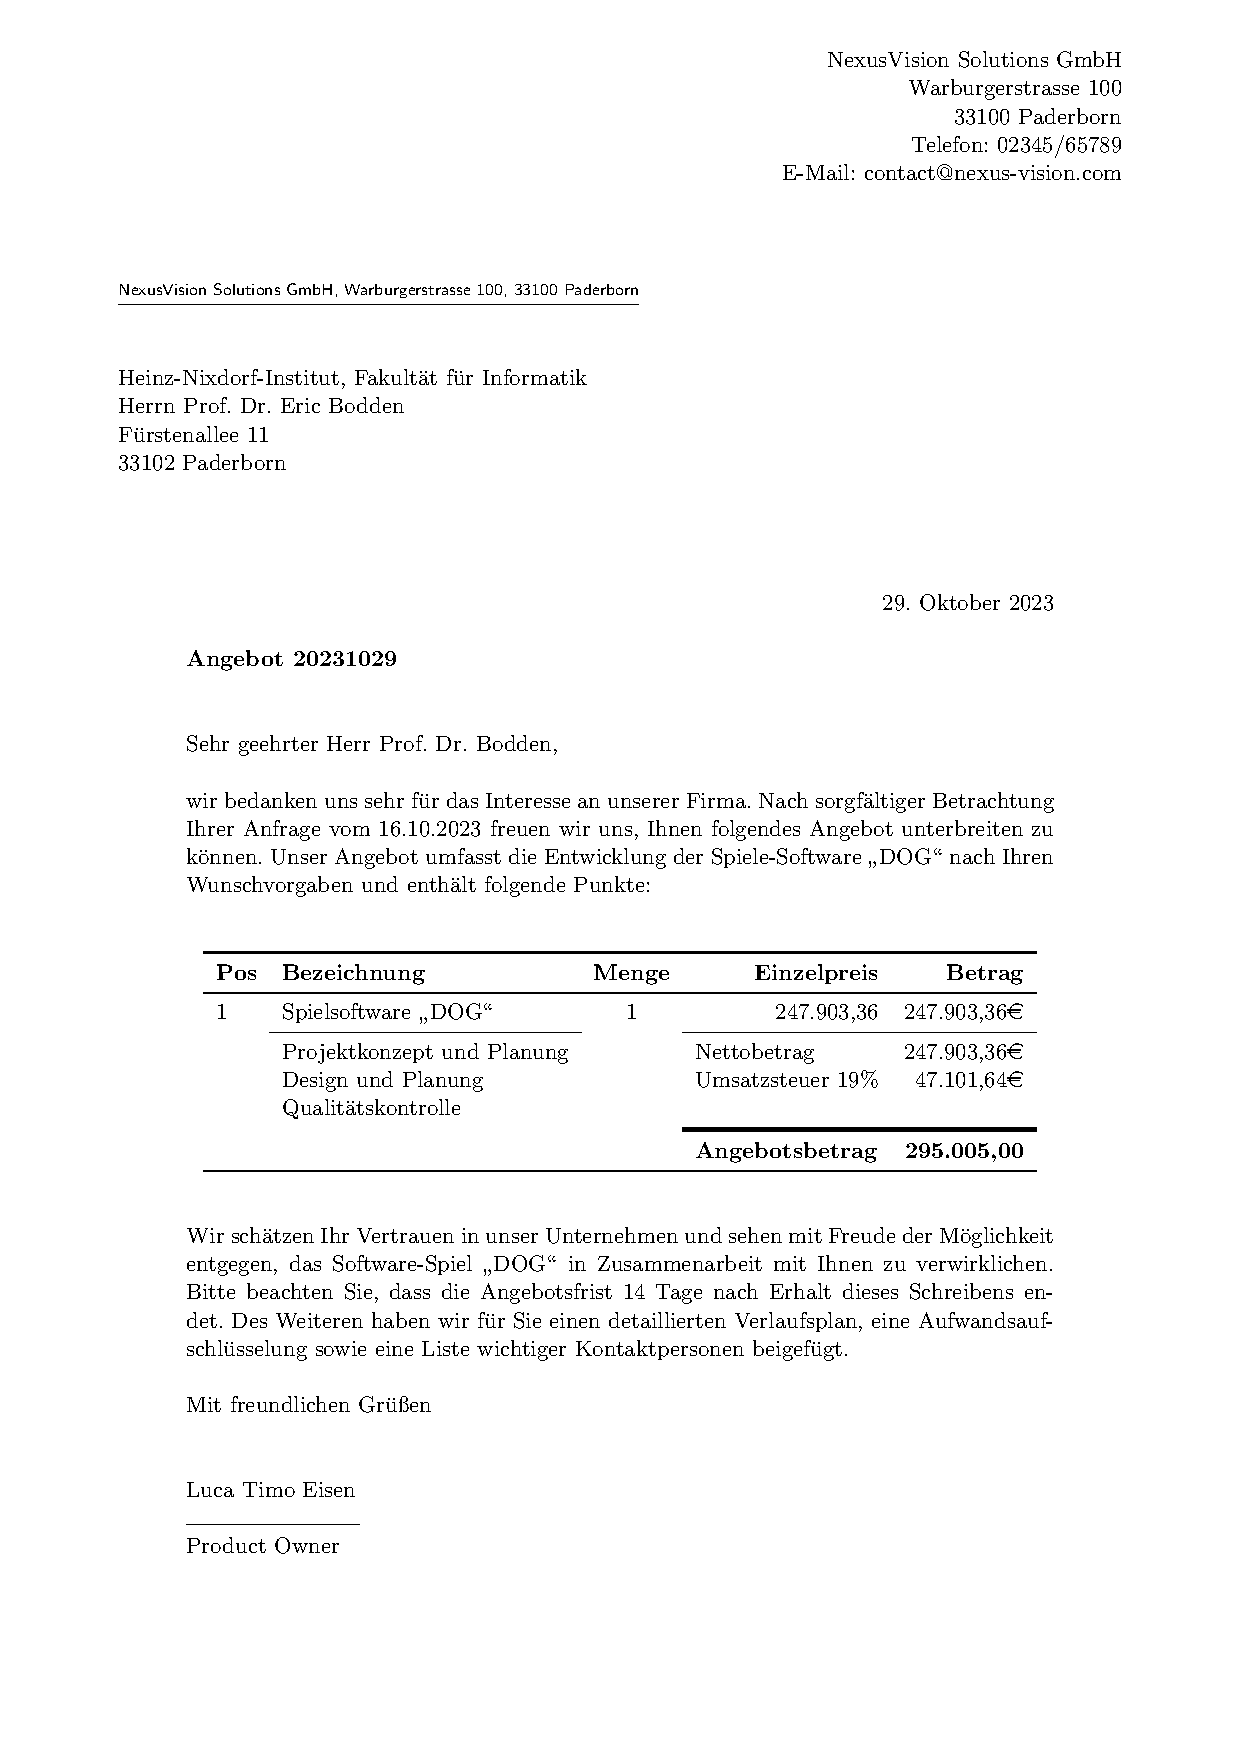
\includepdf{Briefanschreiben.pdf}   %Auf Anschreiben muss noch Seitenzahl entfernt werden
\section{Projektplan}
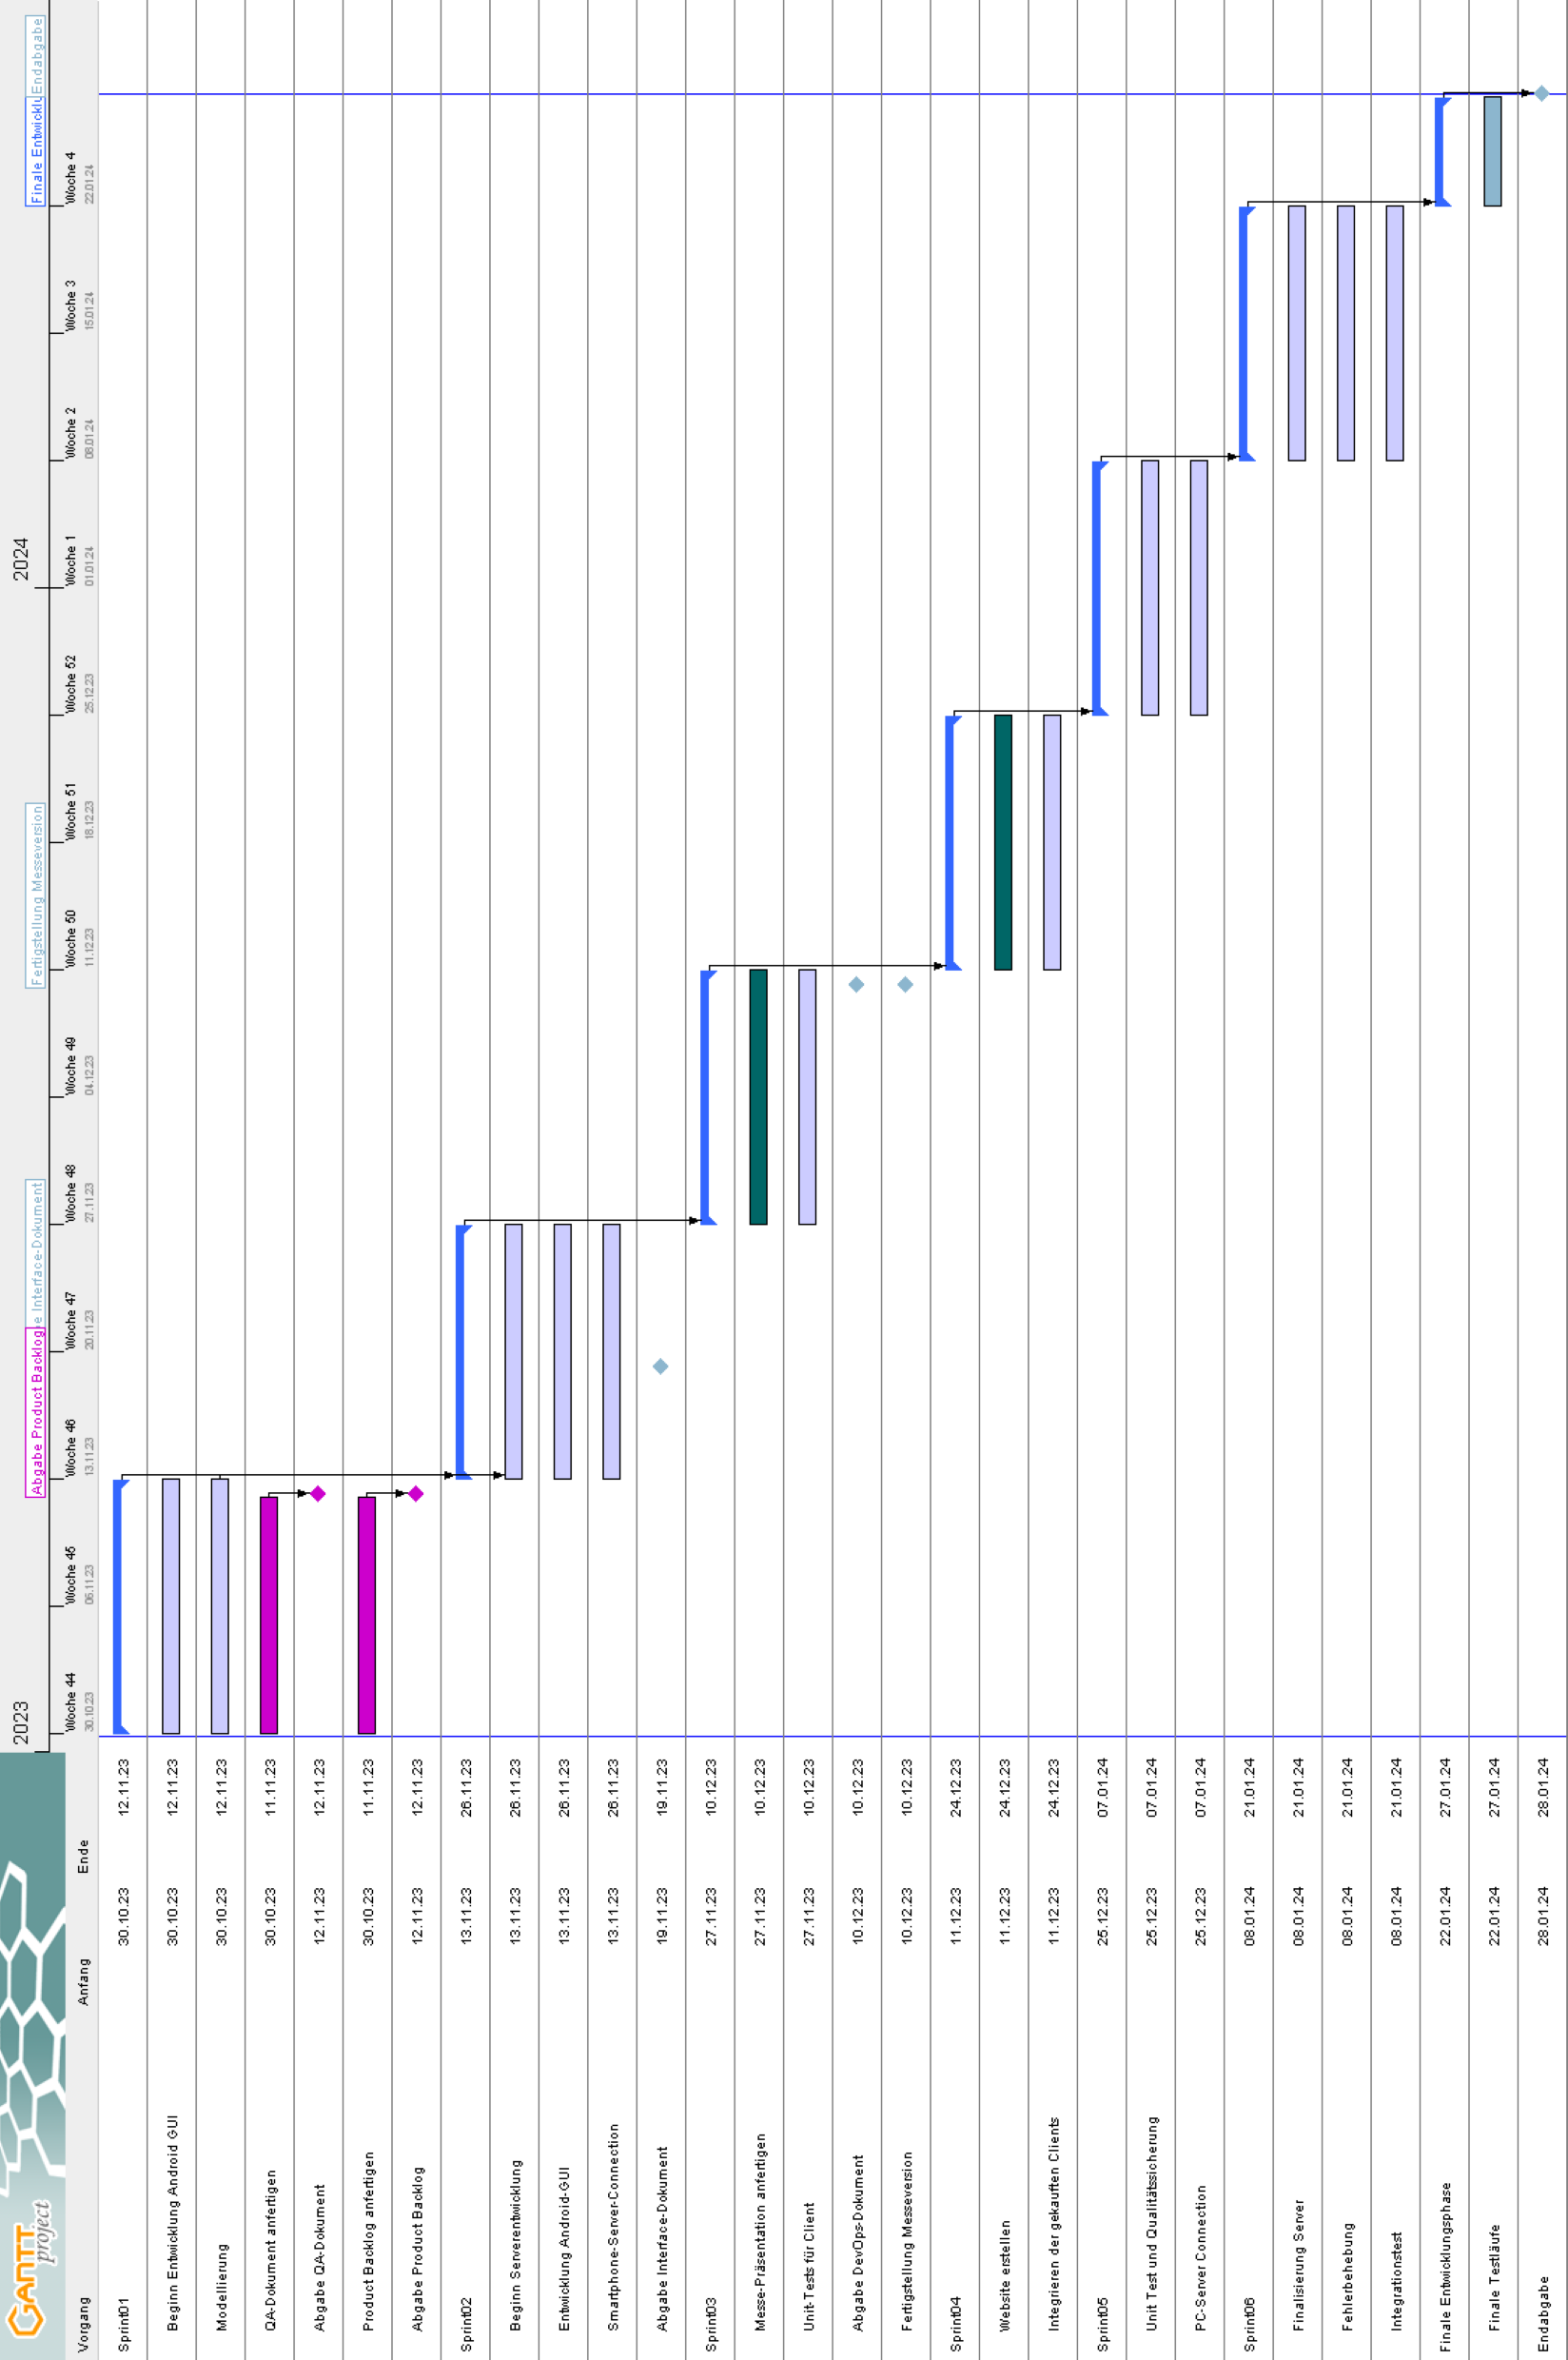
\includegraphics[scale=0.37]{images/Projektplan_DOG_1_Test.png}
\setcounter{page}{1}
\section{Erläuterungen}
\textbf{Entwicklungsumbegung Scrum:}
Um ihren Ansprüchen gerecht zu werden und ihre Anfrage effizient zu bearbeiten, haben wir uns bei diesem Projekt für das agile Entwicklungsmodell Scrum entschieden. \\
%\textbf{Product Backlog-}
%Product Backlog \\

\textbf{\large{\underline{Sprint 1}}} \\
Im ersten Sprint etablieren wir die Grundlage für unser Projekt. Wir modellieren die Anforderungen, starten die Android-GUI-Entwicklung, erstellen ein QA-Dokument und definieren das Produkt-Backlog.\\
\\
\textbf{\large{\underline{Sprint 2}}} \\
In Sprint 2 setzen wir die Entwicklung unseres Projekts fort. Wir beginnen mit der Serverentwicklung, setzen die Entwicklung der Android-GUI fort und implementieren die Smartphone-Server-Verbindung. Dieser Sprint ist entscheidend, da er die Grundlage für die Zusammenarbeit zwischen Client und Server schafft und unsere Anwendung funktionsfähig macht. Durch diese Schritte werden wir unser Produkt stetig weiter vorantreiben, während wir gleichzeitig die Kommunikation zwischen den Komponenten sicherstellen.\\
\\
\textbf{\large{\underline{Sprint 3}}} \\
In Sprint 3 richten wir unseren Fokus auf die Vorbereitung für eine Messepräsentation. Wir erstellen eine Messeversion unseres Produkts, verfassen das DevOps-Dokument und bereiten uns darauf vor, unser Projekt der Öffentlichkeit zu präsentieren. Dieser Sprint ist entscheidend, da er sicherstellt, dass unser Produkt für die Präsentation einsatzbereit ist und unsere Entwicklungs- und Bereitstellungsprozesse gut dokumentiert sind.\\
\\
\textbf{\large{\underline{Sprint 4}}} \\
In Sprint 4 konzentrieren wir uns auf die Erstellung einer Website für unser Projekt und die Integration extern gekaufter Software. Dieser Sprint ermöglicht es uns, eine Webpräsenz für unser Projekt zu schaffen und von extern erworbenen Lösungen zu profitieren, um die Funktionalität unseres Produkts zu erweitern. Durch diese Schritte werden wir eine breitere Präsenz und zusätzliche Funktionalitäten in unser Projekt einbringen, um den Nutzen und die Sichtbarkeit unserer Anwendung zu steigern.\\
\\
\textbf{\large{\underline{Sprint 5}}} \\
Im Sprint 5 liegt der Schwerpunkt auf Qualitätssicherung und der Etablierung der PC-Server-Verbindung. Wir führen umfassende Unit-Tests und Qualitätssicherungsmaßnahmen durch, um die Zuverlässigkeit und Leistung unserer Anwendung sicherzustellen. Gleichzeitig richten wir die PC-Server-Verbindung ein, um die Interaktion mit unserer Anwendung auf verschiedenen Plattformen zu ermöglichen.\\
\\
\textbf{\large{\underline{Sprint 6}}} \\
In Sprint 6 stehen die Serverentwicklung und Qualitätssicherung im Mittelpunkt. Wir finalisieren die Serverentwicklung, beheben Fehler und führen Integrationstests durch. Dieser Sprint markiert einen entscheidenden Schritt in Richtung Produktvollendung, da wir die Serverkomponente abschließen, Fehler beheben, um die Stabilität zu gewährleisten, und sicherstellen, dass alle Teile unserer Anwendung nahtlos miteinander interagieren. Dies ist ein wichtiger Schritt, um unser Projekt für den Produktivbetrieb vorzubereiten.

%\newpage

\section{Aufwandsschätzung}
\begin{center}
\begin{tabular}{llc} 
    \toprule
    Komplexität & Kategorie &  Einflussfaktor \\
    \midrule
    einfach & Externe Ein- und Ausgaben & 20 \\ 
    mittel & Externe Ein- und Ausgaben & 40 \\
    komplex & Externe Ein- und Ausgaben & 60 \\
    einfach & Benutzerinteraktionen & 5 \\ 
    mittel & Benutzerinteraktionen & 25 \\ 
    komplex & Benutzerinteraktionen & 45 \\ 
    einfach & Externe Schnittstellen & 15 \\
    mittel & Externe Schnittstellen & 35 \\ 
    komplex & Externe Schnittstellen & 55 \\ 
    einfach & Interne Dateien & 10 \\ 
    mittel & Interne Dateien & 30 \\ 
    komplex & Interne Dateien & 50 \\
    \bottomrule
\end{tabular}
\end{center}

Die Implementierungen wurden nach Kategorie und Komplexität gewertet und dementsprechend wurde jeder ein Einflussfaktor zugeschrieben. Mit Hilfe der Function-Point-Methode wurde die Bewertung der einzelnen Entwicklungen modifiziert, wobei sich die Abweichungen zum Ursprungsaufwand um maximal 30\% unterscheiden. 

\begin{equation}
    FP_{bew.} = FP_{unbew.} \cdot (\frac{Einflussfaktor}{100} + 0,7)
\end{equation}

Pro Stunde Arbeitsaufwand haben wir Kosten in Höhe von 142,00 Euro berechnet. Die berechneten Gesamtkosten können sich auf Grund von Inflation und Zukauf von zusätzlicher Software oder unvorhersehbaren Faktoren um bis zu +/-13\% abweichen.


\begin{center}
    \begin{tabular}{lcccc} 
        \toprule
        Komplexität & FP_{ungewichtet} &  Einflussfaktor & FP_{gewichtet} & Kosten (in \euro{})  \\ 
        \midrule
        Android GUI entwickeln & 150 & 25 & 142.5 & 20.235,00 \\ 
        Smartphone-Server-Connection & 100 & 35 & 105 & 14.910,00\\
        Smartphone Backend & 100 & 55 & 125 & 17.750,00\\
        Server-Implementation & 250 & 55 & 312.5 & 44.375,00\\ 
        Design Patterns & 100 & 30 & 100 & 14.200,00\\ 
        Docker-Containerisierung & 50 & 30 & 50 & 7.100,00\\
        Ausrichter entwickeln & 50 & 25 & 47.5 & 6.745,00\\ 
        Entwicklung eines KI Spielers & 150 & 45 & 172.5 & 24.495,00\\ 
        PC-GUI & 150 & 25 & 142.5 & 20.235,00\\ 
        PC-Server Connection & 150 & 35 & 157.5 & 22.365,00\\ 
        PC Backend & 150 & 35 & 157.5 & 22.365,00\\ 
        Erstellen einer Webseite & 150 & 20 & 135 & 19.170,00\\ 
        QA-Dokument anfertigen & 100 & 10 & 80 & 11.360,00\\ 
        DevOps Dokument anfertigen & 150 & 30 & 150 & 21.300,00\\ 
        Messe-Präsentation anfertigen & 100 & 30 & 100 & 14.200,00\\ 
        Abschlusspräs. anfertigen & 100 & 30 & 100 & 14.200,00\\ 
        \midrule
        Gesamt & 2000 & - & 2077.5 & 295.005,00\\
        \bottomrule
    \end{tabular}
\end{center}
\newpage
\section{Kontakt}
Sollten bei ihnen Fragen zu bestimmten Bereichen aufkommen, dann ist das Team von NexusVision jederzeit für sie erreichbar.

\begin{center}
    \begin{tabular}[h]{lll}
        \toprule
        \textbf{Zuständigkeit} & \textbf{Kontaktperson} & \textbf{E-Mail} \\
        \midrule
        Scrum Master & Bengiamin Keller & kellerb@mail.uni-paderborn.de \\
        Product Owner & Luca Timo Eisen & leisen@mail.uni-paderborn.de \\
        Qualitätsmanager &  Danny Joschua Gehse & dgehse@campus.uni-paderborn.de\\
        Testmanager & Felix Werner & felixwr@mail.uni-paderborn.de \\  % sind doppelte Rollen in Ordnung ?
        Produktmanager & Bengiamin Keller & kellerb@mail.uni-paderborn.de\\
        Dokumentationsmanager & Farah El Azzouzi-Yücel & farah-ey@mail.uni-paderborn.de\\
        Werkzeugbeauftragter & Felix Werner & felixwr@mail.uni-paderborn.de\\
        Komitee-Mitglied & Mattes Hachmeyer & hachmeye@mail.uni-paderborn.de \\
        \bottomrule
    \end{tabular}
\end{center}

%\newpage


%\pagenumbering{arabic}
\printindex

\end{document}